\chapter{Architecture in Distributed Applications}
\label{ch:architecture}

This chapter is about architectural styles for distributed applications. Considering the architecture of any application is extremely important to ensure that the application can be effectively maintained and expanded in the future. Architecture for distributed applications has moved through several phases: monolith, service oriented architecture (SOA), and microservice.

\note{
“ This chapter is about architectural styles, application architectures, and architecture patterns. A style describes how to implement a specific architecture, while an architecture pattern explains how to address a specific concern within an architecture but is broader than a design pattern. I suggest you not get too hung up on the differences, but just understand that DDD can reside at the heart of a lot of surrounding architectural influences.”
Excerpt From: Vernon, Vaughn. “Implementing Domain-Driven Design.”

We need to emphasize that there are many ways of doing architecture and many reason for doing particular architectures. Functional and non-functional requirements
}


\section{Domain Driven Design}
The DDD term was coined by Eric Evans in his book of the same name from 2004\cite[preface]{evans2004domain}. Evans works with the notion that any complex domain should be partitioned into smaller subdomains, making it possible to comprehend the different subdomains and how a good solution can be created in that part of the domain. Models express a deep understanding of a particular subdomain, defining a model makes it possible to talk about the domain internal in a development team and externally with other development teams or customers. The model is a product of careful analysis of the domain, and should be reflected in the implementation, so that the analysis of the domain is visible in the code. This makes it possible to understand the implementation, and helps when maintaining and updating the application\cite[p.~2]{evans2004domain}.

Evans deems it very important that a model is kept simple, emphasizing the need for having several subdomains with their own model. Having a single model for a large system is not feasible or cost-effective\cite[p.~331]{evans2004domain}. By introducing what he calls \textit{Bounded contexts}, a models applicability is limited. A model is created in relation to a certain context, and this context will vary between each subdomain, concepts will likely occur in several subdomains, but might have very different meanings. Sharing a model across bounded contexts might hide the fact that there is a discrepancy in how the model is utilized, which can cause buggy and unreliable software, that is hard to understand. By limiting usage of a model, by explicitly defining bounded contexts, teams have a clear understanding of what is consistent across context and how it relates to their context\cite[p.~331]{evans2004domain}. Figure \ref{fig:architecture_bounded_context} show a domain with three bounded contexts and five subdomains. The different subdomains have dependencies across bounded context boundaries, indicating integration points.

\begin{figure}[!htb]
  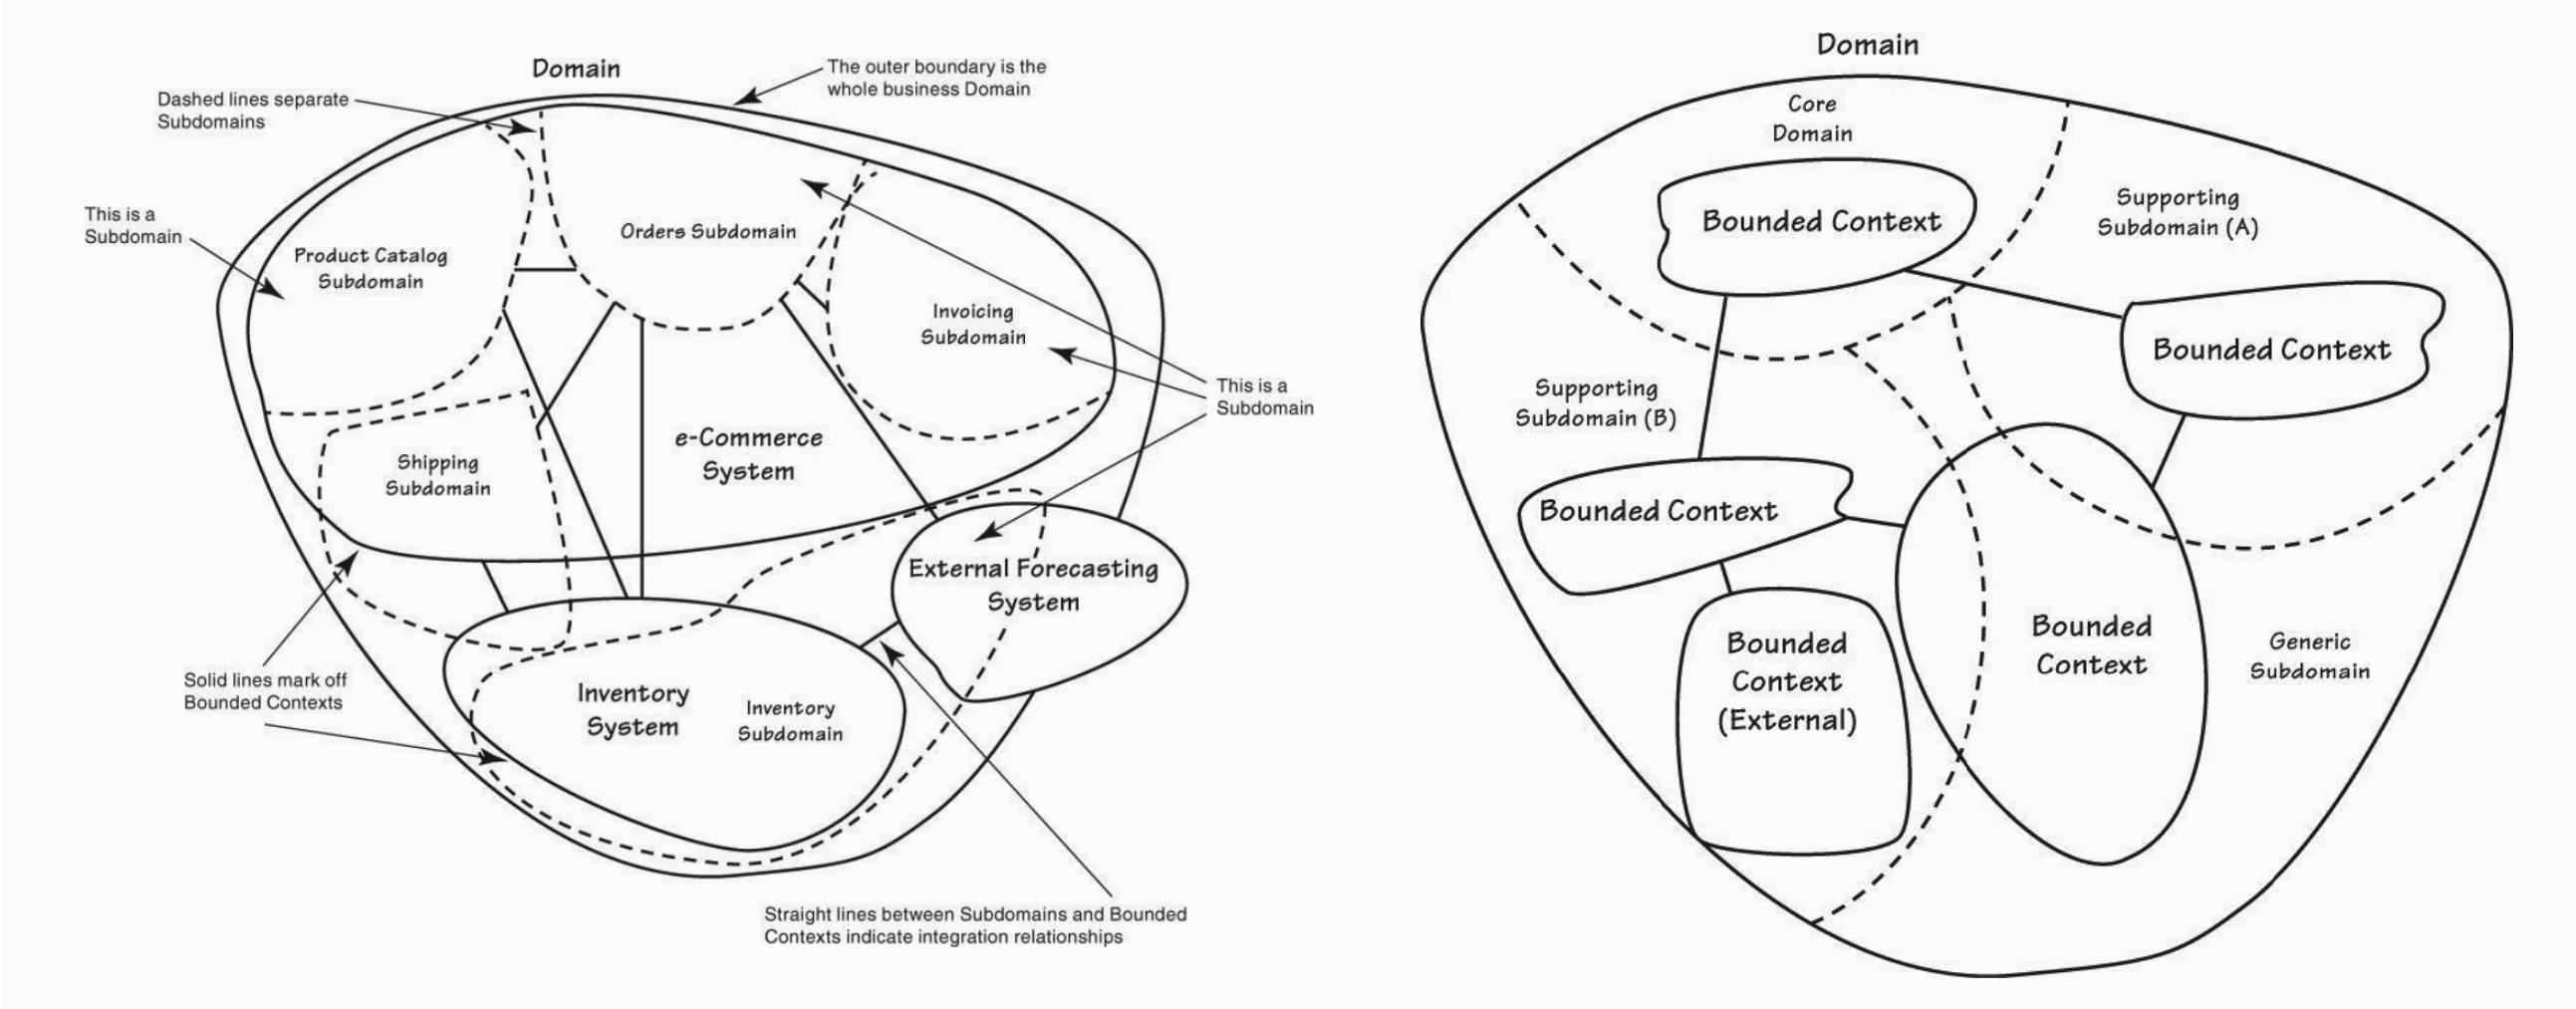
\includegraphics[scale=0.28]{architecture_bounded_context}  
  \caption{An example of bounded context}
  \label{fig:architecture_bounded_context}
\end{figure}


\citeauthor{fowler2014microservices} describes the usability of DDD when designing distributed applications:

\begin{quote_highlight}
DDD divides a complex domain up into multiple bounded contexts and maps out the relationships between them. This process is useful for both monolithic and microservice architectures, but there is a natural correlation between service and context boundaries that helps clarify, and as we describe in the section on business capabilities, reinforce the separations\cite{fowler2014microservices}.
\end{quote_highlight}\\

\citeauthor{fowler2014microservices} emphasize how DDD is usable, generally when designing applications, also mentioning how separation between bounded contexts is more explicit when using microservices, highlighting one of the key features of the architecture. Reducing the risk of sharing model across bounded contexts.

\section{Monolithic}
The word monolith describes a application that exists as an single unit. By having the entire application as a single entity, the source code can be developed and managed together, giving multiple short term advantages\cite[p.~68]{long2017cloud}. Functionality can easily be added on top of a existing code base, giving the many advantages of low level programming language constructs. Communication can be done internally, between processes, not relying on non-deterministic network communication channels. 
According to \citeauthor{fowler2014microservices} enterprise web applications are often created as a monolith, consisting of three main parts: a client-side user interfaces, a shared common database management systems and a monolith server-side applications. The server-side application is a large and complex application, packed into a single executable. The application binds interface and database together, executing domain logic based on user input, retrieving and updating data as needed. 
As the application grows in size, immediate advantages fade. The code base reaches a size where small changes in one part of the application might incur unforeseen changes in other parts. Centralizing the application decreases risk of failure, but at the same time forces development teams to coordinate changes, making sure breaking changes are not introduced\cite[p.~68]{long2017cloud}. 
According to Eric Evans having a single and unified model for a large system is not feasible nor cost-effective, and have several potential pitfalls if legacy code is updated by several teams simultaneously. Coordination might halt the project completely. The unified model may not be sufficient for some parts of the application, forcing functionality in elsewhere. Having a unified model leads to a very complex model that tries to encapsulate all aspects of the particular domain, making it difficult to use and therefore defeating the purpose\cite[p.~331]{evans2004domain}.

\subsection{Netflix -- the Transition away from the Monolith}
According to \citeauthor{meshenberg2016microservices} Netflix previously had a monolithic implementation of their website. Each team would contribute a JAR file, that would be gathered into a single WAR file, that was deployed on a internal infrastructure. According to \citeauthor{meshenberg2016microservices}, this kind of architecture is very unreliable, mentioning that any issue introduced in either of the JAR files would be propagated onto all copies of the single service site executable. More importantly, the old architecture had a single relational database management system (RDBMS), creating a single point of failure\cite{meshenberg2016microservices}. Netflix experienced a outage, where their central RDBMS failed and caused wide system failure, resulting in four days with downtime. According to \citeauthor{meshenberg2016microservices} this event started the Netflix transition from a monolith to a microservice architecture.

\note {
The client-side user interface consists of HTML pages, with some underlying javascript files. The database is a shared among all applications in the enterprise, implemented as a relational database, containing tables for the entire business domain. The server-side application is a monolith, binding interface and database together, executing domain logic based on user input and retrieving and updating data as needed. The server-side application is a single executable.

"To start explaining the microservice style it's useful to compare it to the monolithic style: a monolithic application built as a single unit. Enterprise Applications are often built in three main parts: a client-side user interface (consisting of HTML pages and javascript running in a browser on the user's machine) a database (consisting of many tables inserted into a common, and usually relational, database management system), and a server-side application. The server-side application will handle HTTP requests, execute domain logic, retrieve and update data from the database, and select and populate HTML views to be sent to the browser. This server-side application is a monolith - a single logical executable[2]. Any changes to the system involve building and deploying a new version of the server-side application." \cite{fowler2014microservices}
}

\section{Service-Oriented Architecture}
\comment{still missing}

\section{Microservices}
Microservice architecture gives an application composed of many small intercommunicating services. Each individual service has a well defined and limited functionality and a well defined interface for external communication. Services communicate with each other through their interfaces and together they achieve a overarching business goal\cite[p.~2]{newman2015microservices}. A comparison between a monolithic and microservice architecture is shown on Figure \ref{fig:architecture_microservice_definition}, showing they key difference between the two architecture types. Microservices are independently deployable, whereas the monolith scales 1:1, giving less flexibility. 

Having small and independently deployable services makes it possible to update services as teams identify problems or add new features. This supports agile software development, giving the flexibility and agility that the monolithic implementation lacks. By having small services, creating a modular, easy readable and understandable architecture is easier. Each service can be developed, tested and deployed independently, by the team creating it, minimizing the need for coordination between teams\cite{kniberg2014spotify}.

At the same time microservices introduce more complexity. By having individual services, each service has it's own life cycle and can potentially fail. Microservices makes it necessary to have increased automation when deploying, monitoring and maintaining system health\cite{meshenberg2016microservices}.


\begin{figure}[!htb]
  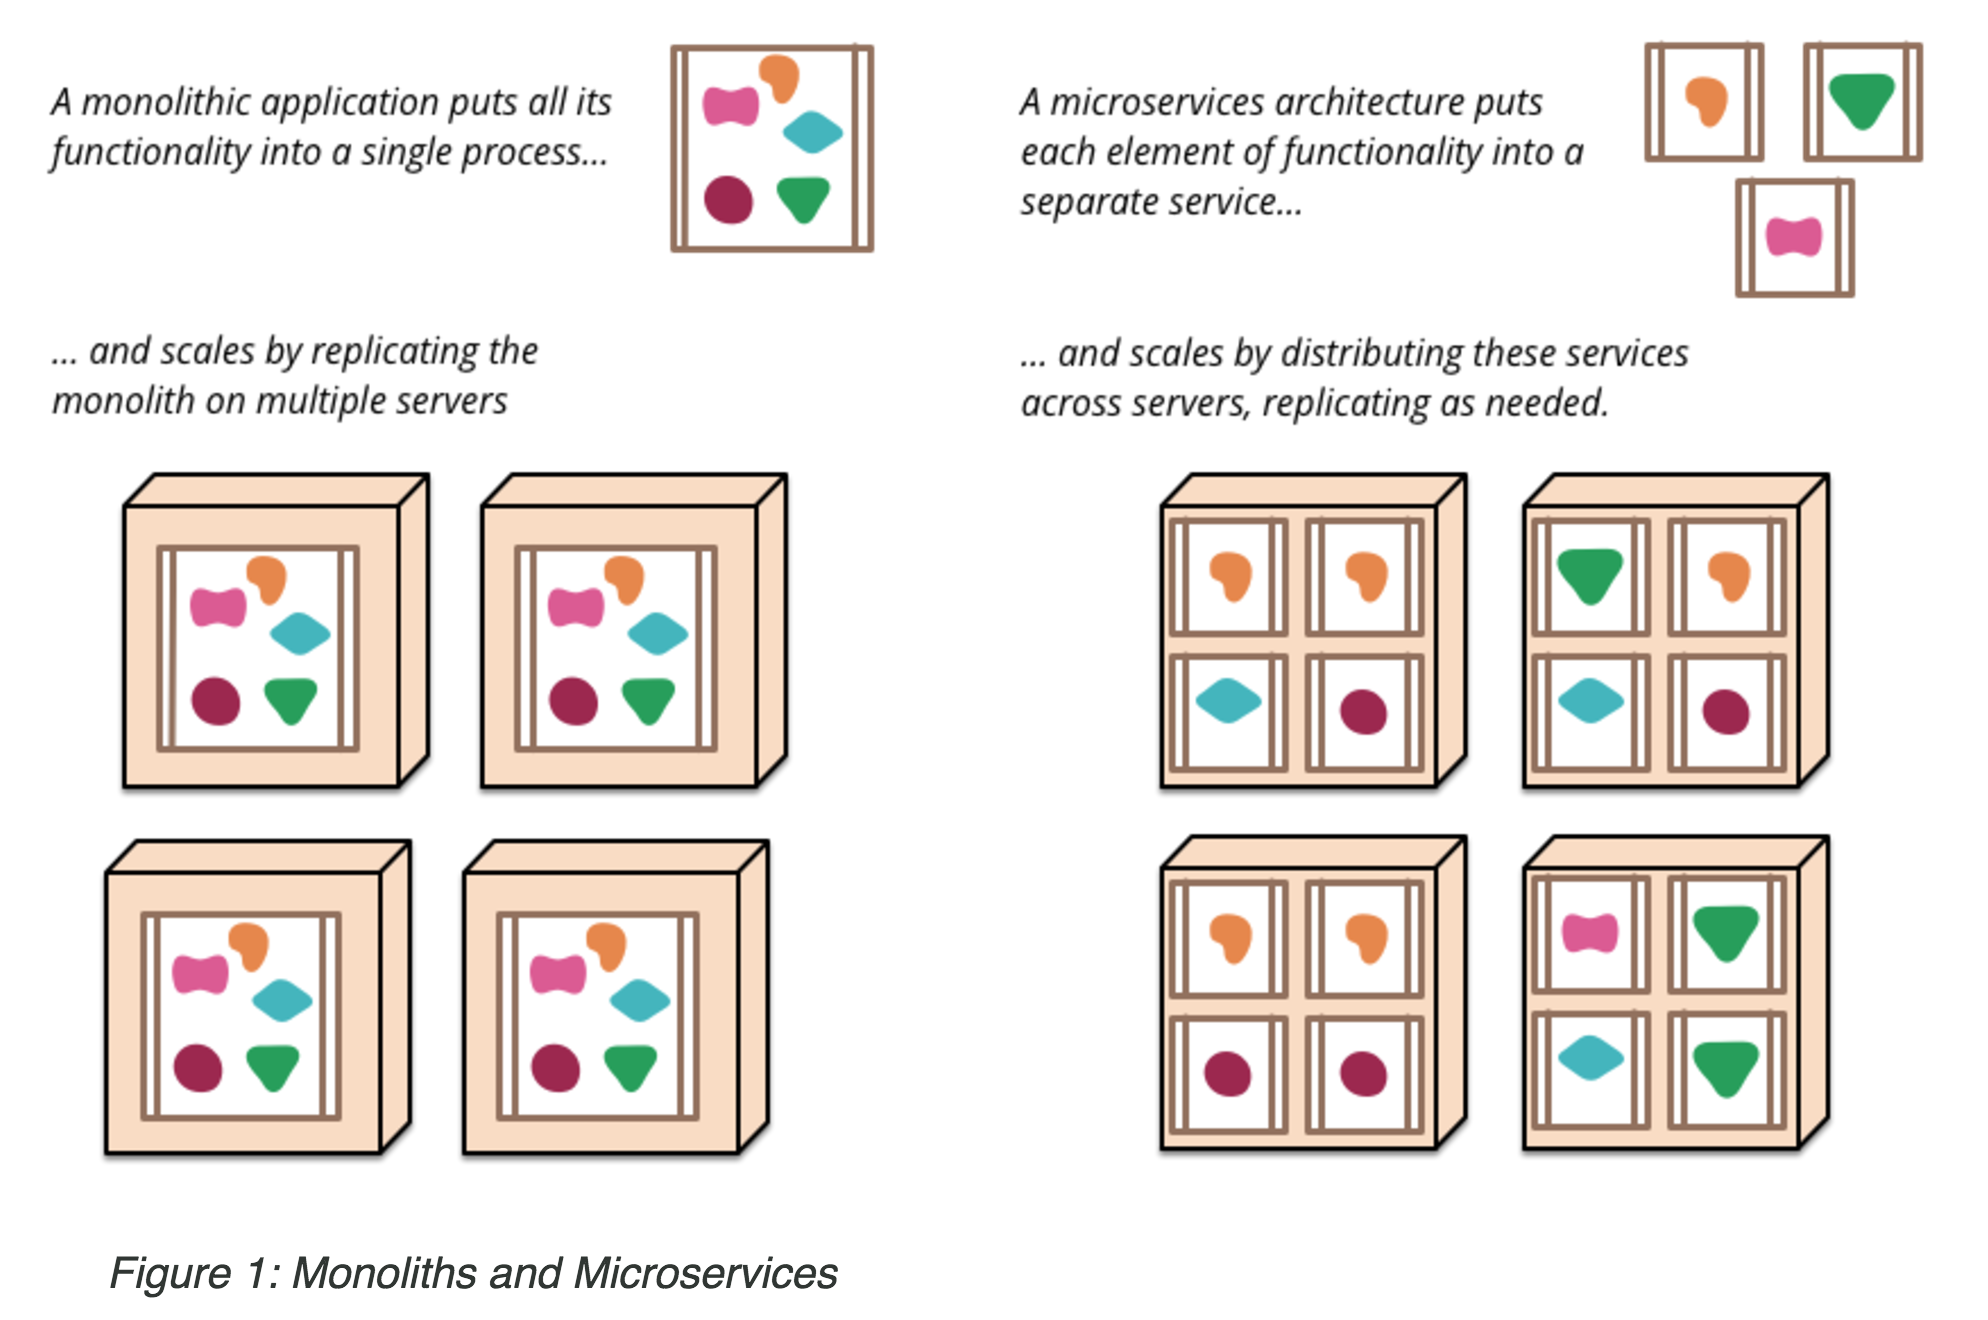
\includegraphics[scale=0.24]{architecture_microservice_definition}  
  \caption{Monolith and Microservice architectures compared}
  \label{fig:architecture_microservice_definition}
\end{figure}

\subsection{Defining characteristics}
\note{
As the microservice architecture was created out of a need for reducing complexity and improving agility and reliability\cite[p.~68]{long2017cloud}, different companies started developing microservice architectures independently.
}
There is a series of defining characteristics for services in a microservice architecture, which should be followed to avoid pitfalls when utilizing microservices. These characteristics describe what teams utilizing microservices often times do, there is no definitive definition of what a microservice architecture is.

\subsubsection*{Componentization via Services}
Componentization is used to decouple parts of an application, so that a service is only responsible for limited amount of highly related functionality\cite{morgantini2013whatAreMicroServices}. The componentization can initially be created by analysing the domain and identifying bounded contexts\cite[p.~31]{newman2015microservices}, each bounded context contains information only important internally in the context. 
The external important information is therefore made available through a interface, while internally important information is hidden from outsiders, simplifying boundaries.

By using services for componentization, a explicit interface is created, hindering tight coupling between components. Explicit remote call mechanisms are often used to facilitate communication between components. Communication through remote calls incur some overhead, forcing communication interfaces to be on high abstraction levels, making them more awkward to use than in process calls.

\subsubsection*{Splitting around Business Capabilities}
Services are organized around business capabilities, by analysing the domain carefully, each service can be limited in size and functional requirements. Each service implements all functionality to fulfil the identified requirements for that part of the business area, potentially consisting of multiple processes, developed and deployed together. A service could implement a application process having a underlying database exclusively used for that application process\cite{fowler2014microservices}.

\subsubsection*{Well Defined and Simple Communication Channels}
Keeping logic out of the communication method is important when developing microservices. Inspired by UNIX implementation, microservice architecture tries to delegate the entire concern of applying logic to the service implementations. When a service receives a request it applies its logic as appropriate and produces a response. The communication is often done with HTTP request-responses, defining the communication interfaces with a REST protocol\cite{fowler2014microservices}.

\subsubsection*{Decentralized Governance}
By decentralizing governance and organising around business capabilities, each service can be build with technology that fits well with solving the problem.
\note{Kunne potentielt tilføje hvordan team skills også kan splittes ud, samt hvordan det gør teams i stand til at sidde forskellige steder og arbejde med det samme}

\subsubsection*{Decentralized Data Management}
Services often have their own data store, decentralizing data management. Each service has the data that is relevant for that service, and not more. 

\note{Potentielt gør brug af Martin Fowler artikel "PolyglotPersistence", der snakker om brug af NoSQL teknologier}

\subsubsection*{Automation of Deployment}
Microservices infer a lot of operational complexity, as there are many services to deploy and monitor. The use of infrastructure automation techniques is necessary, improving insight into the quality of newly developed software, and reduce the time it takes to move new features from development to production\cite{newman2015microservices}. This is often achieved with build pipelines know from Continous delivery (CD), a build pipeline is seen on figure \ref{fig:architecture_microservice_build_pipeline}.

\begin{figure}[!htb]
  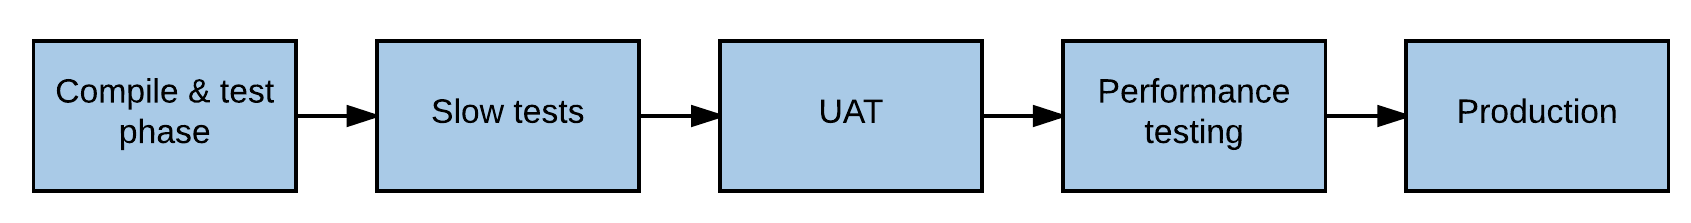
\includegraphics[scale=0.26]{architecture_microservice_build_pipeline}  
  \caption{Build pipeline(lend from Sam Newmann)}
  \label{fig:architecture_microservice_build_pipeline}
\end{figure}

\note {
\subsubsection*{Independently Deployable Services}
Each service is independently deployable, making it possible to add and update functionality in each service as needed.
}

\subsection{Derived qualities}
Microservices in it self presents a lot of benchmark benefits, giving possibility to control capacity, introduce redundancy and solve single point of failure issues, a microservice architecture improves overall application resilience if utilized correctly. At the same time microservices introduces additional complexity, because services has to communicate with dependent services using non-deterministic communication channels. This in turn has the effect of highlighting otherwise transparent challenges with integration points, causing engineers utilizing microservices to be more resilience aware, expecting failure between services. In a monolith implementation, a library dependency used in process might introduce new possible error states or undefined behaviour, but in this context software engineers tend to be less aware of the possible errors this dependency could incur. When having very clear interfaces with dependencies, engineers tend to take more precautionary measures. These measures are not directly measurable, but help create a more resilient system. 

\subsubsection*{Design for Failure}
A challenge with using services as components is the inherent complexity of communication over the wire, when two separate services need to communicate. In turn this highlights the existing pitfalls with every integration points, that exists even in a monolith architecture.

\subsubsection*{Sophisticated Real-Time Monitoring}
When designing many independent services, it is necessary to have sophisticated monitoring and logging, in order to control that services are running correctly. This enables engineers to know if any action needs to be taken to restore a fully functional system, or if service was automatically restored.